\section{Rauschen}
Rauschen ist ein physikalischer Effekt, der auf Grund der Bewegung und der Quantisierung der Ladungsträger entsteht. Deterministische Signale addieren Amplitude, stochastische Rauschquellen addieren Rauschleistung.

Dabei ist Rauschen \textbf{Mittelwertfrei} $\overline{v_n}(t) = \frac{1}{T}\int_{T}^{}v_n(t)dt = 0$. Die \textbf{Rauschleistung} aber ungleich Null $\overline{v_n}(t)^2 = \frac{1}{T}\int_{T}^{}v_n^2(t)dt \neq 0$

\subsection{Widerstandsrauschen}
Jeder Widerstand rauscht, unabhängig vom Stromfluss.
\begin{center}
	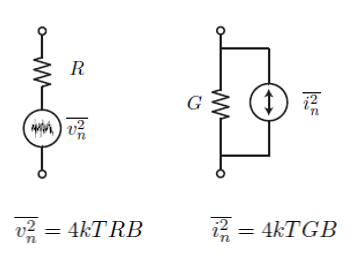
\includegraphics[width=0.6\columnwidth]{Images/widerstandsrauschen}
	\begin{tabular}{ll}
		Rauschspannungsdichte & $e_n = \sqrt{\overline{v_n^2}}$ \\
		Boltzmann-Konstante & $k = 1.38\cdot 10^{-23}J/K$ \\
		Abs. Temperatur & $T$ \\
		Widerstand & $R$ oder $G = \frac{1}{R}$ \\
		Bandbreite & $B = f^+ - f^-$
	\end{tabular}
\end{center}

\subsubsection{Spannungsteiler}
Spannungsteiler $Div = \frac{R_2}{R_1 + R_2}$ mit Leistungsdichte $S$\\
\begin{align*}
	S_{R1} &= 4kTR_1 \\
	S_{R2} &= 4kTR_2 \\
	S_{R1\_Vout} &= 4kTR_1 \cdot \left(\frac{R_2}{R_1 + R_2}\right)^2 \\
	S_{R2\_Vout} &= 4kTR_2  \cdot \left(\frac{R_1}{R_1 + R_2}\right)^2  \\	
	S_{Vout} = S_{R1\_Vout} + S_{R2\_Vout} &= \underline{\underline{4kT\cdot \frac{R_1R_2}{R_1 + R_2}}}
\end{align*}
Dies ergibt eine Rauschspannungsdichte von $e = \sqrt{S_{Vout}}\frac{nV}{\sqrt{Hz}}$

\subsubsection{Serie- und Parallelschaltung}
Äquivalente Schaltung von Spannungsteiler. Ersatzwiderstand gesehen vom Ausgang $R_T = R_2 + R_1||R_3$
\begin{center}
	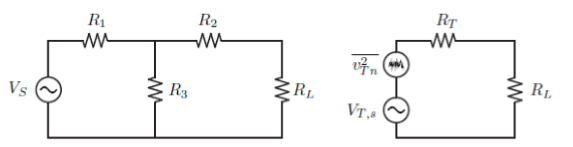
\includegraphics[width=0.6\columnwidth]{Images/rauschen_serie_parallel}
\end{center}
\[
\overline{V_T^2} = 4kTR_TB = 4kT(R_2 + R_1||R_3)B
\]


\subsection{Opamp Rauschen}
Die Rausch-Spannungsdichte $e_n$ oder auch $V_{noise}$ ist bei typischen Opamps $25\frac{nV}{\sqrt{Hz}}$.
\begin{center}
	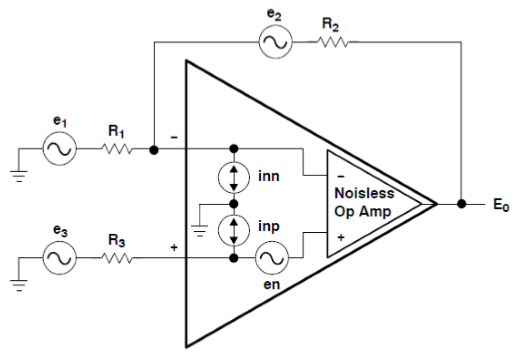
\includegraphics[width=0.6\columnwidth]{Images/opamp_rauschen}
\end{center}
Die Ausgangs-Rauschspannung $E_0$ wird berechnet mittels \underline{Superposition.} Eine weitere wichtige Eigenschaft ist die \textbf{Rausch-Bandbreite} $ENB$. Sie wird berechnet mit der \textbf{Verstärkungs-Bandbreite-Produkt} $GBP$ und dem Verstärkungsfaktor $A$
\[
ENB = \frac{GBP}{A}\frac{\pi}{2}
\]
Mittels der Spannungsdichte $E_{wnd}$ (aus Datenblatt) und $ENB$ kann der Effektivwert des weissen Rauschen berechnet werden $E_{op\_wn} = E_{wnd}\sqrt{ENB}$

Wenn Bandbreite $>>$ Noise Corner Frequency ist, kann Pink-Noise vernachlässigt werden (gilt für Bandbreite $>10kHz$).
\[
V_{noise} = \sqrt{4kT\cdot R_2\cdot A\cdot ENB + e_{w}^2 \cdot A^2 \cdot ENB}
\]
~\\
tl;tr: Grosse Widerstände bewirken grosse Rauschspannungen, reduzieren dafür Stromverbrauch. Optimal sind Widerstände die etwa gleich wie Opamp rauschen.

